
\chapter{Algorithm Partitioning}
\label{chap:Algorithm Partitioning}

%Summary: add on the idea of the partitioner to reconfigurable instrumentation rather than the partitioning coming from a person we can use a computer to optimize this
%describe linear program in detail
%describe and defend design choices/heuristics/approximations
%Goal: show how to do cost-driven partitioning of a design
%for now �cost� and �performance� are still variables
%State: intro to ILP can be written now. documenting the actual ILP for this application will be done after the analysis/results

%TODO: Place
%Cluster abstraction
%Treat platforms as cluster nodes
%Assume all platforms elements are attached to a switch
%Assume a full crossbar network
%Fully connected network
%Often necessary in radio astronomy
%Try to determine the best mapping based on some cost metric

After coming up with an instrument description, it is necessary to determine how that instrument will be implemented in hardware. 
I use Integer Linear Programming (ILP) to model and solve this problem. 
As described in Section \ref{Related Work:Tuning}, ILP is a powerful technique for defining and solving optimization problems.
In this chapter I explain how the ILP is defined based on the dataflow model and the techniques used to make sure the program can be solved quickly.

%Treat platforms as cluster nodes
%Assume all platforms elements are attached to a switch
%Assume a full crossbar network
%Fully connected network
%Often necessary in radio astronomy
%Try to determine the best mapping based on some cost metric

%Results are repeatable
%Easy to add user input
%Easy to �build out� a cluster, just add (a limited amount of) free hardware




%But� it�s NP-Hard to solve optimally
%Current ILP benchmarks run 100k variable problems in hours
%Beyond that size, problems become infeasible
%ILP runtime highly sensitive to
%ILP solver (underlying algorithm) � 100k problem infeasible with one tool vs <3 minute solution with another 
%Problem structure
%We can help the algorithm out for large designs
%Reduce number of variables (combine blocks)
%Early stopping (non-optimal result)
%Guided optimization

\section{Variables}
The variables in the ILP are represent the optimal mapping for the system.
%and the cluster architecture.   TODO: explain this
Ultimately, the ILP determines which platforms should be used, and what part of the algorithm should get implemented on each platform.
This is achieved by having the ILP consider some platform, and assume it can instantiate at most $n_p$ copies of that platform.
We will call a copy of the platform a board. 
Each board must have some variables that determine which computation blocks get mapped to it. 
For some board $i$, the number of computation blocks of type $b$ that get mapped to it is represented by the variable $n_{i,b}$.

A solution to the ILP, with each of the $n_{i,b}$ variables filled in, gives a complete specification of the optimal mapping for that instrument.

\section{Constraints}

%Constraints are used to determine a valid mapping (ex. total bandwidth mapped to a link must be less than total link bandwidth) 
%Constraints (resources)
%I/O

The constraints serve two purposes.
First, they ensure that no resource is overmapped, so that the amount of hardware the ILP generates will be sufficient to do the computation required.
Second, they make sure that the correct design gets implemented.


\subsection{Platform Resources}
Any resource some board that gets used by mapping computation blocks to that board must be accounted for in the linear program. 
This is abstracted in the ILP using by adding single constraint for each resource.

\subsubsection{Resource Limitations}
For some resource, $r$, we use our performance model of each block to assess how much of the resource is used up by each block type. 
The percentage of the resource $r$ required by some block type, or utilization, is represented by a constant (not a variable), $r_{p,b}$, where $p$ represents the platform, and $b$ represents the block type. 
Multiplying the resources required for a specific block type by the number of blocks needed on that specific board determines the total percent of resource $r$ block type $b$ will require on the board. 
Summing over all of the block types determines what percent of resource $r$ is used in the final design, which gives us the final format of the constraint needed to ensure that some resource $r$ is not overmapped on board $i$:

\begin{equation}
\sum_{b\in Blocks} n_{i,b} r_{p,b} \leq 1
\end{equation}

Each resource will require a separate constraint in the ILP of this form. By ensuring that the total utilization of each resource required is less than 100\%, we guarantee that there are enough resources to allow all the blocks mapped to that board to complete their tasks. 

\subsubsection{Dataflow Model Constraints}
After getting assurance that no resources are overused, it is important to verify that the correct design was implemented. 
The resource utilization on the value of $n_{i,b}$, but there are is an additional constraint on these variables.
Namely, that the correct number of blocks actually get implemented. 
This adds a simple constraint to each block type:

%TODO: check that this can't be geq (probably can't because of certain types of links)
\begin{align}
\sum_{board in boards} n_{board,block type} == n_{block type}
\end{align}

The total number of blocks of a certain type should be equal to the number of blocks of that type we actually need in the design. 
 
%#check that all blocks are allocated        
%prob+=lpSum(board_blocks[blocktype,currentplatform,currentboard] for currentplatform in range(numplatforms) for currentboard in range(numboards)) >= numblocks[blocktype]



\subsection{Network Resources}

\begin{figure}[ht!]
  \centering
     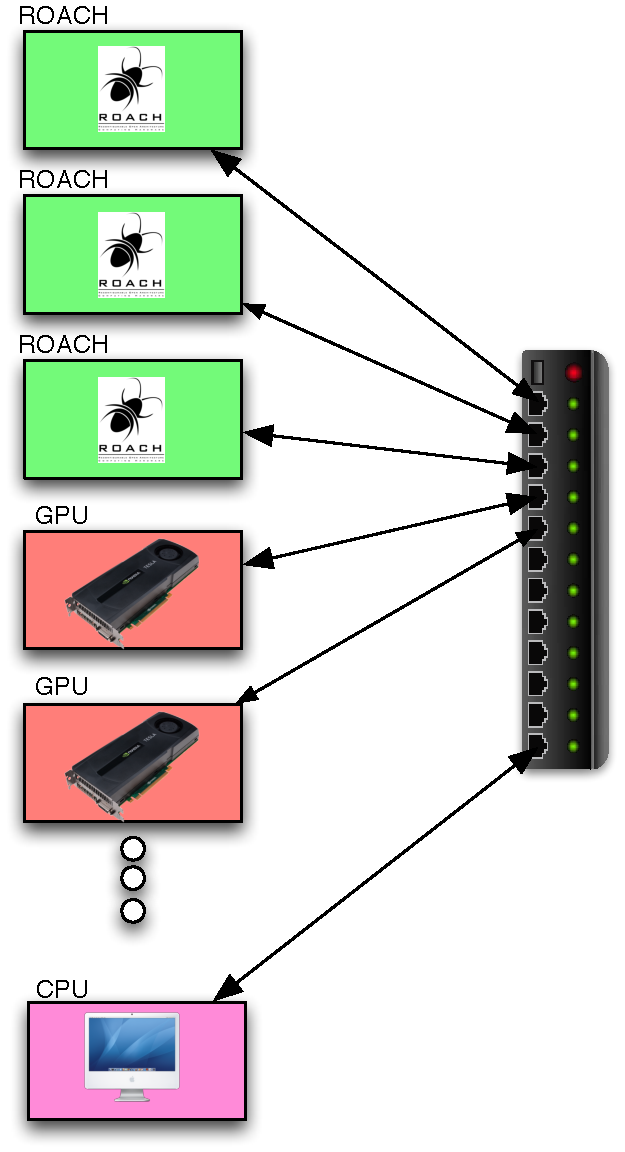
\includegraphics[width=0.3\textwidth]{Images/C5/cluster_instruments.pdf}
  \caption{Full-Crossbar Interconnect Model}
  \label{fig:C5/cluster_instruments.pdf}
\end{figure}

The ILP does not design the network topology. 
While it would be possible to design the network using an ILP, %TODO: add ref
this would add unnecessary complexity to the program (therefore increasing the runtime) with little gain.
As described in Section \ref{Related Work:Radio Astronomy}, most radio astronomy applications require a full-crossbar interconnect at some point, because many computational blocks have an all-to-all or one-to-all communication pattern.
Rather than have the ILP redesign the same topology over and over, we simply assume this interconnect exists and every board can communicate with every other board directly over a fixed-bandwidth link.



Figure \ref{fig:C5/cluster_instruments.pdf} shows an example of this topology. 
Each board gets connected to the same switch and can communicate with any other board on the switch, regardless of the platform type. 

\subsubsection{Bandwidth Limitations}
Even a fixed network topology, there still are communication constraints that must be taken into account in the ILP.
While there might be a link available between each pair of boards, the bandwidth into and out of these boards is limited. 
Consider Figure \ref{fig:C5/cluster_instruments.pdf} again.
Suppose every other board in the cluster needed to stream 10 Gbps of data to the CPU board, but it is only connected to the switch via a single 10 Gbps link. 
%TODO so what?
There are additional constraints to ensure that the input and output bandwidths are not exceeded.


In order to write these constrains, we must first determine how many blocks need to communicate with a block that is not located on the same board. 
We introduce new variables $nr_{i,b}$ to represent the number of blocks of type $b$ on board $i$ that need to receive data from the cluster, and, similarly, $ns_{i,b}$ to represent the number of blocks of type $b$ on board $i$ that need to send data to the cluster. 
Given the amount of data some computational block type takes as input and the number of those blocks on the board, we can multiply them together to determine the amount of input bandwidth that computational block type will require. 
Summing over every block type determines the total amount of input bandwidth needed by all the computational blocks on the board, creating a constraint that the total required bandwidth must be less than or equal to the total available input bandwidth.
The constraint on output bandwidth is calculated the same way, generating a pair of constraints for each board, one restricting the total amount of input bandwidth, and another restricting the total amount of output bandwidth. 

%#check that we don't exceed the input/output bandwidth
%prob += lpSum(blockinputbw[blocktype]*num_receive_data[blocktype,currentplatform,currentboard] for blocktype in range(blocktypes)) <= platforminputbw[currentplatform]
%        prob += lpSum(blockoutputbw[blocktype]*num_send_data[blocktype,currentplatform,currentboard] for blocktype in range(blocktypes)) <= platformoutputbw[currentplatform]
\begin{align}
\sum_{b\in Blocks} nr_{i,b} bw\_in_{b} \leq bw\_in_{p} \\
\sum_{b\in Blocks} ns_{i,b} bw\_out_{b} \leq bw\_out_{p}
\end{align}


%TODO: this might be better explained in chapter 4, putting it here so the relevant info is available
%TODO: explain better
\subsubsection{Connection Constraints}
First, we observe that the these variables must be bounded by $0$ and $n_{i,b}$, since there cannot be a negative number of blocks that need to communicate, and the number of blocks of type $b$ that need to communicate can't exceed the number of blocks physically on the board. 
Next, we must take into account the structure of the algorithm to determine whether or not a given block needs to communicate with a separate board. 


While the constraints on the total input and output bandwidth might seem simple, ensuring the values for $nr_{i,b}$ and $ns_{i,b}$ are sane requires additional constraints.
Suppose we know we have 2 types of blocks: $A$, and $B$. 
$A$ is a source of data, meaning it does not data from any computation block. 
Similarly, block $B$ is a sink, with no data to send to another block.
Regardless of how many $A$ and $B$ blocks get placed on platform $i$, none of the $A$ blocks will need to receive data and none of the $B$ blocks will need to send data. 
Knowing that $A$ is a source and $B$ is a sink tells us that $nr_{i,A}=0$ and $ns_{i,B}=0$. 

In order to appropriately define the linear program, it is first important to look at the different ways the computational blocks in a design may need to communicate, and create appropriate constraints. 
We must revisit the connection types introduced in Section \ref{High Level Toolflow:Dataflow Model}, and determine how the different types of links affect the linear program.



When two blocktypes are linked via a `one-to-one' connection, communication is required when the number of $A$ blocks is different than the number of $B$ blocks on a single board. 
When there are more $A$ blocks then $B$ blocks, $n_{i,A}>n_{i,B}$, the number of $A$ blocks that need to send data to the cluster is $n_{i,A}-n_{i,B}$ and none of the $B$ blocks on that board need to receive data from the cluster. 
In the opposite case, $n_{i,A}<n_{i,B}$, and the none of the $A$ blocks need to send data to the cluster, but $n_{i,B}-n_{i,A}$ blocks of type $B$ will need to receive data from the cluster.
Both of these cases are captured by the same pair of constraints:

\begin{align}
ns_{i,A} \geq n_{i,A}-n_{i,B} \\
nr_{i,B} \geq n_{i,B}-n_{i,A} 
\end{align}

When $n_{i,A}-n_{i,B}$ is non-negative, we are guaranteed that we will not underestimate $ns_{i,A}$, and when $n_{i,A}-n_{i,B}$ is negative, $ns_{i,A}$ will be forced to at least 0 because of the lower limit on the variable. 
 

%TODO: fix linear program to calculate this
Setting the $ns$ and $nr$ variable is a little more complicated for the `all-to-all' case, and requires the implementation of some conditional logic in the linear program.
When any of the $B$ blocks are not on the board $i$, then every $A$ block must send data to the cluster, and $ns_{i,A} = n_{i,A}$.
Otherwise, none of the $A$ blocks need to send and $ns_{i,A}=0$.
Similarly on the receive side, if any of the $A$ blocks are not of board $i$, $nr_{i,B}=n_{i,B}$, otherwise $nr_{i,B}=0$.
The conditional logic is easily implemented in an ILP, as describe in X. %TODO: add reference to ILP tips and tricks

When a block must send to or receive data from multiple different block types, the is constraint the same way an `all-to-all' connection gets constrained. 
If any of the blocks it must link to reside outside the board, it is assumed that all of the data must be sent over the link to the cluster.

%TODO: some numbers on why this is ok
Implementing the ILP this way results in an overestimation of the required bandwidth. 
In the case where $ns_{i,A} = n_{i,A}$, it's true that every block of type $A$ will need to send some data.
However, they might not need to send the full bandwidth $bw\_out_{A}$ to the switch, since some portion of the data sent by an $A$ block may be required by $B$ blocks residing on the same board. 
A more exact version of this calculation would also take into account the smaller bandwidth, but due to the complexity and rarity of this case the approximation is sufficient.
As described in Section \ref{Related Work:Radio Astronomy}, many architectures have this type of connection but there very few cases where the $A$ and $B$ blocks connected this way reside on the same board. 

\section{ILP Implementation}
In software, the ILP can be generated automatically using the dataflow model contained in an instrument object.
The generic Instrument class has a single function, called runILP() that iterates through the dataflow model, creating variables and constraints, determines the cost model depending on what the user wants to optimize for and runs an ILP solver to generate an optimal mapping.
Adding on to the instrument creation example in Section \ref{High Level Toolflow:Instrument Definition}, we show how the user can create and map an instrument using only two function calls in the following code.

\lstinputlisting[language=Python,
    %caption=My Class,
    label={runilp.py},
    breaklines=true,
  ]{code/C5/runilp.py}

\section{Performance Modeling}                    

The data that the ILP uses to measure resource utilization must come from a preexisting performance model.
These models can take a number of forms. 
Benchmarks of compiled and running code provide the best information, but are also time consuming to obtain if they don't already exist and they require a real implementation of the block.
Estimates are faster to obtain but won't be as accurate. 
Nevertheless, many DSP blocks have predictable performance and a performance estimate based on similar benchmarks can be very reliable.

\begin{figure}[ht!]
  \centering
    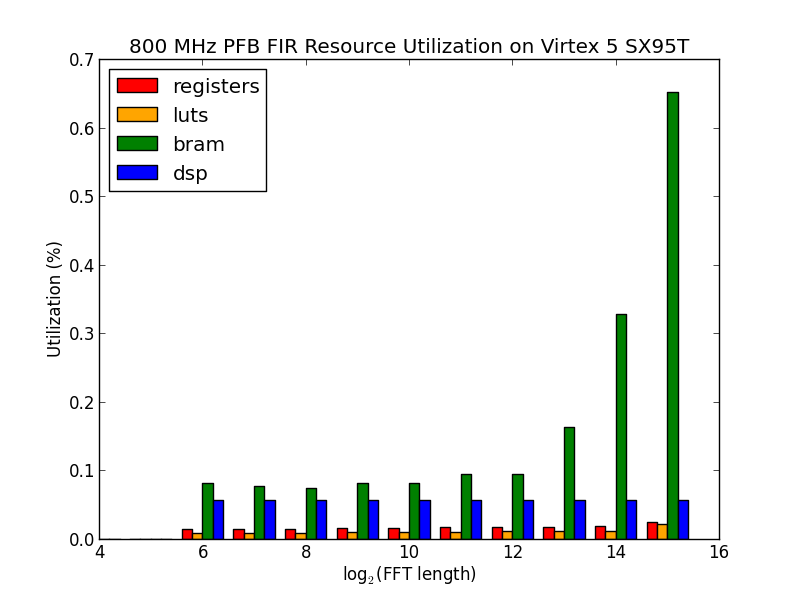
\includegraphics[width=0.75\textwidth]{Images/C6/pfb_bench.png}
     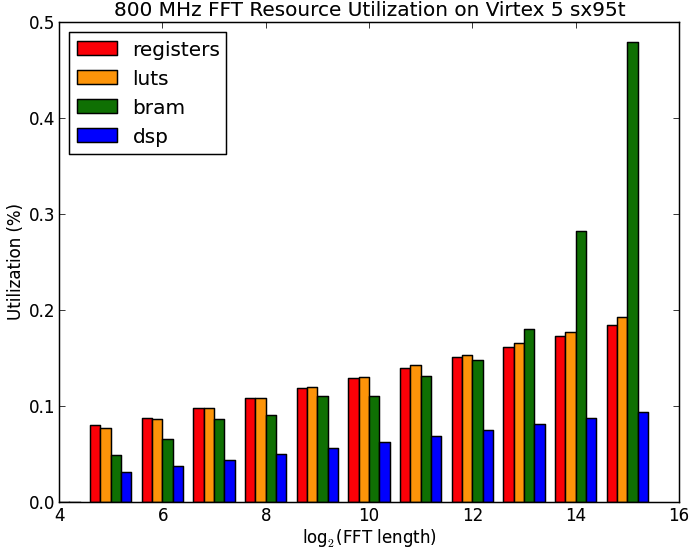
\includegraphics[width=0.75\textwidth]{Images/C6/fft_bench.png}
  \caption{PFB FIR and FFT benchmark data on the Virtex V SX95T}
  \label{fig: C6/fpga_bench.png}
\end{figure}

Benchmarks of the mapped design or running code serve as a very accurate way to assess performance.
Figure \ref{fig: C6/fpga_bench.png} shows the type of benchmarks that would be useful for an FPGA block, measuring utilization of available FPGA resources.
The graphs show the utilization of registers, LUTs, BRAMs and DSPs used on the Virtex 5 SX95T. 
The top graph is the data for an 800 MHz FIR filter with 4 taps, and the bottom shows utilization for an 800 MHz FFT.
Getting the performance model for a specific block simply requires a looking up the FFT size in the graph.

\begin{figure}[ht!]
  \centering
    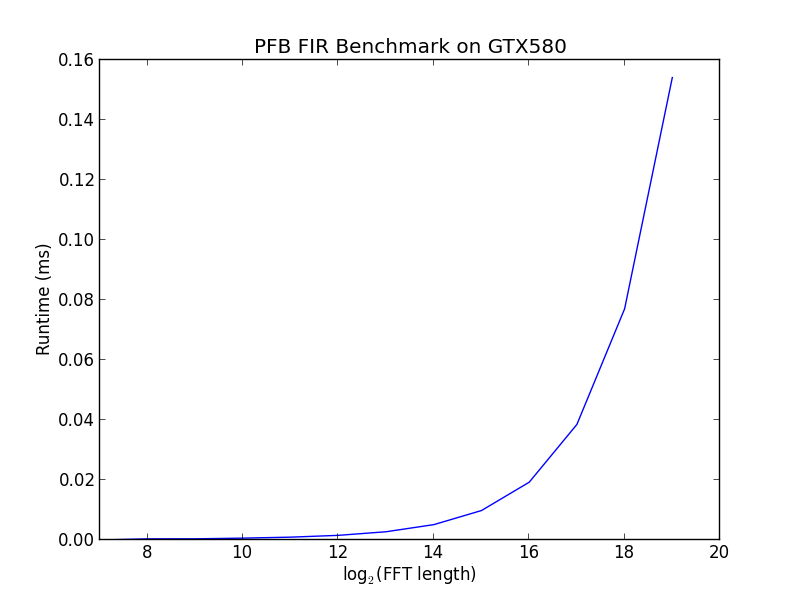
\includegraphics[width=0.75\textwidth]{Images/C6/pfb_gpu_bench.png}
    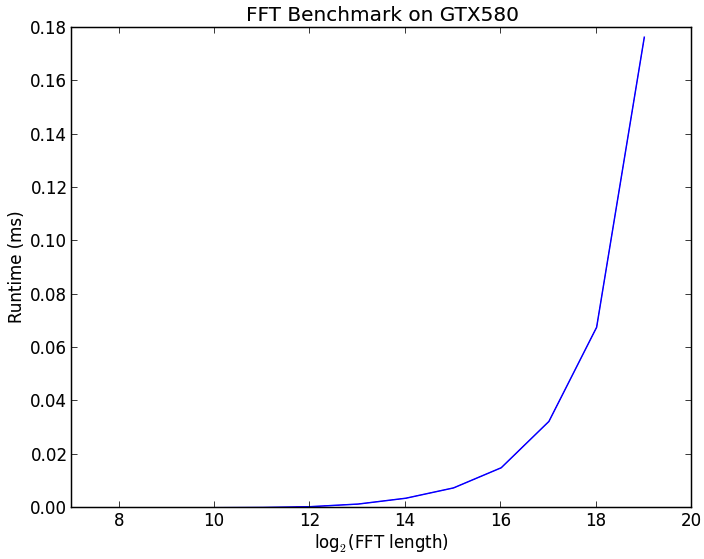
\includegraphics[width=0.75\textwidth]{Images/C6/fft_gpu_bench.png}
  \caption{PFB FIR and FFT benchmark data on the GTX 580}
  \label{fig: C6/gpu_bench.png}
\end{figure}

Similarly, Figure \ref{fig: C6/gpu_bench.png} has benchmarks for the same blocks, FIR filter above and FFT below, but these are tested on a GTX 580 GPU. 
These benchmarks measure the runtime of each function. 

Many papers also provide these kinds of benchmarks, making it easy to get accurate numbers without installing or running the code.
The xGPU paper has a number of graphs demonstrating kernel performance that can be used directly as an ORCAS benchmark, which will be shown in Chapter \ref{chap:Analysis}.

%\begin{figure}[ht!]
%  \centering
%    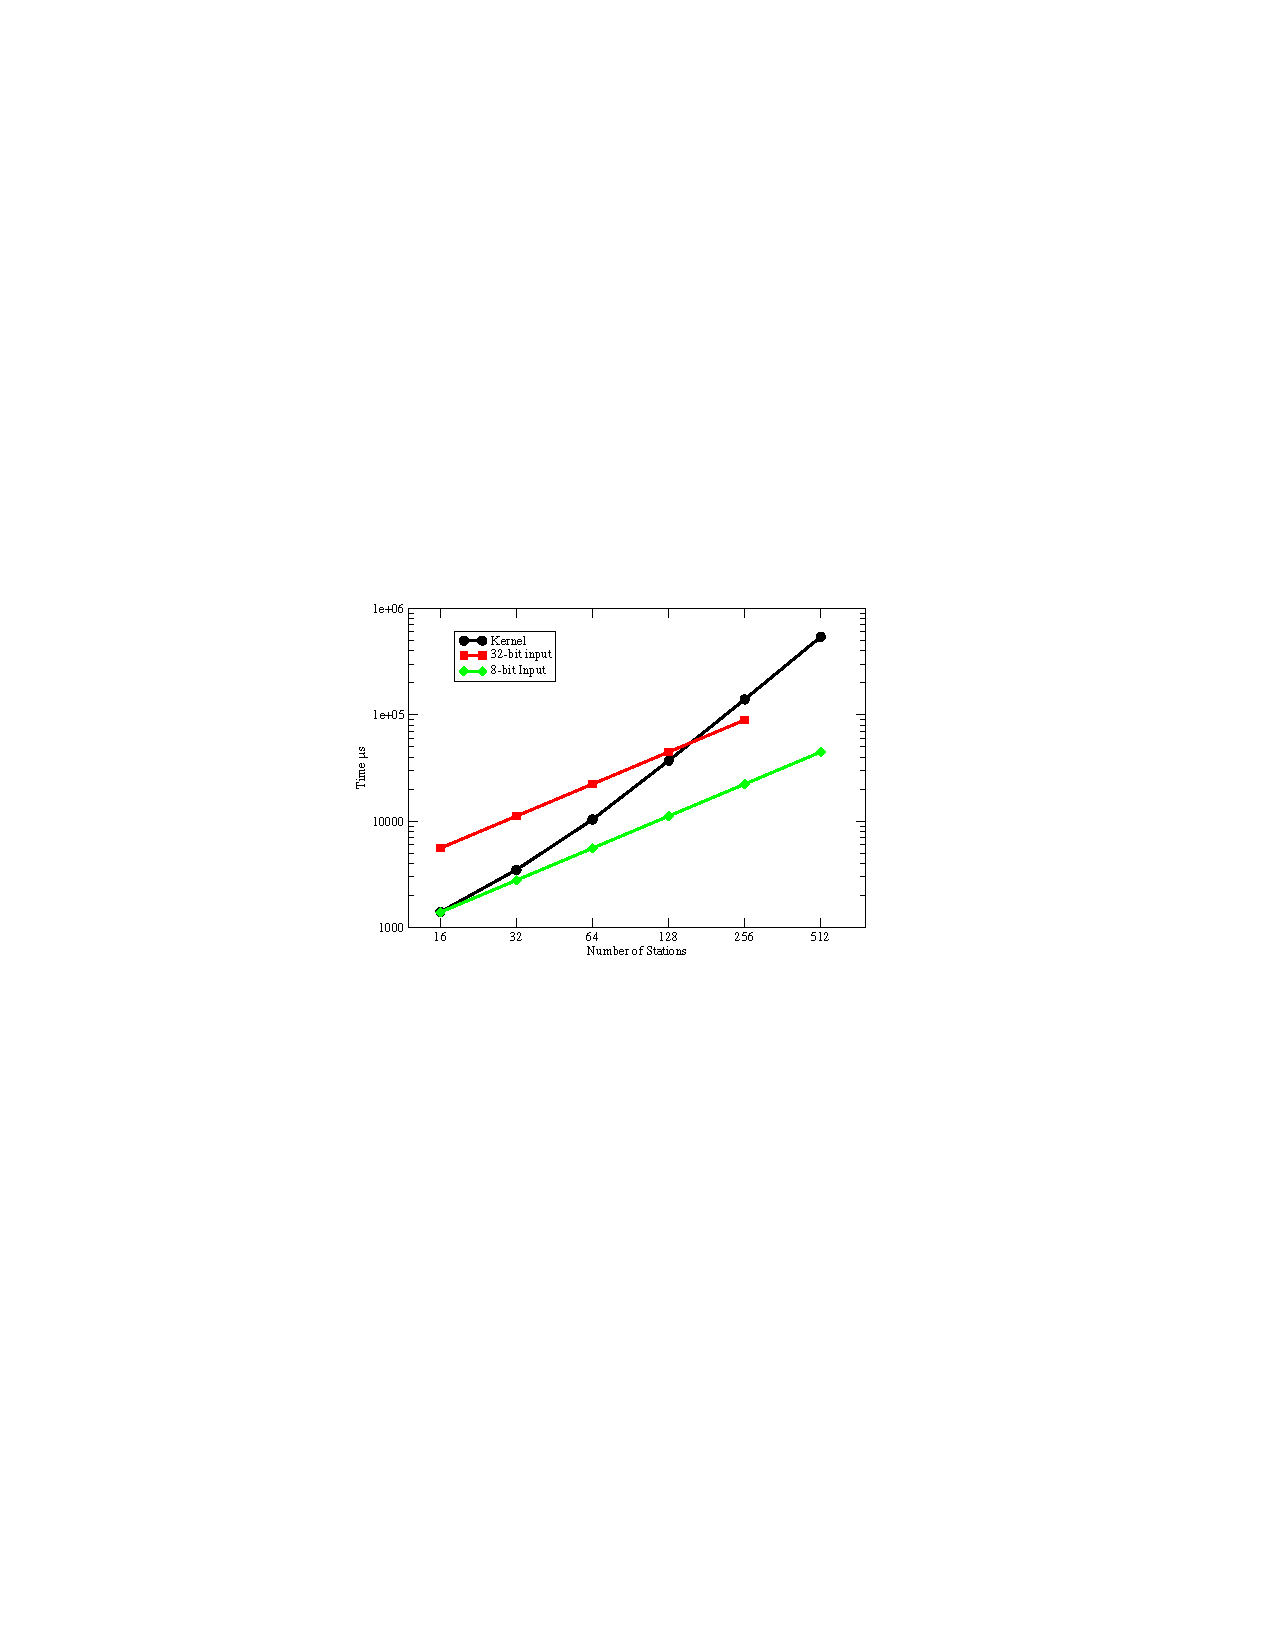
\includegraphics[width=\textwidth]{Images/C6/gpuxperformance.pdf}
%  \caption{xGPU benchmarks on}%TODO: check board for this
%  \label{fig: C6/gpuxperformance.pdf}
%\end{figure}

Performance data can also be represented using formulas. 
Figure \ref{fig: C6/fpga_bench.png} clearly shows some predictable trends in the FIR and FFT utilization.
Primiami, et al turned this predictability into a set of equations that determine the requisite resources with a set of formulas \cite{Primiani:2011vz}.

We can also use existing benchmarks to project how a block might perform on newer technology.
In FPGAs, we notice the number of resources required for a block remains nearly constant between different chips.
Table \ref{tab: C5/compare_resource} shows the resource utilization of an 800MHz 32k channel FFT on three chips from three different generations, the Virtex 5 SX95T, Virtex 6 SX475T, and Virtex 7 VX980T.
Aside from the number of LUTs, which slightly dropped between the Virtex 5 and Virtex 6, the number of resources required remains very stable across chips.
Although the utilization will change, because different chips will provide different amounts of resources, recording the number of resources required on one chip makes it possible to predict the utilization on another chip.

\begin{table}
\begin{tabular}{| l | l | l | l | l | l |}
\hline  
\textbf{Resource} & Virtex 5 SX95T & Virtex 6 SX475T & Virtex 7 VX980T \\
\hline  
Registers & 10881 & 10789 & 10788 \\
LUTs  & 11358 & 9632 & 9773 \\
36k BlockRAM & 100 & 100 & 100\\
18k BlockRAM & 30 & 30 & 30  \\
DSPs & 60 & 60 & 60 \\
\hline  
\end{tabular}
\caption{Comparative Resource Utilization of a 32k Channel 800 MHz FFT}
\label{tab: C5/compare_resource}
\end{table} 

Similarly projections can be made with new processor technology. 
Even if a new technology is not yet available to buy, a conservative and optimistic estimate of the speedup can be used to generate a conservative and optimistic estimate of the instrument cost using that new technology. 

%TODO: put this somewhere
%PASP has proven useful in many applications by itself, but the goal of automatically generating a spectrometer for any cluster requires more than just a reconfigurable FPGA design. 
%It is difficult to determine what size the subbands or the cluster should be without knowing how much data the target servers can receive and process.
%Our benchmarking tools are designed to quickly determine how much bandwidth a server is capable of handling so the PASP parameters can be set appropriately.

%We have developed a general purpose benchmark to test the networking capability of a server. 
%This test uses an FPGA design to generate 10 gigabit Ethernet packets and transmits them to the server under test.
%The FPGA design has a runtime programable packet size and packet rate. 
%The packet size is set to the largest size allowed by the server and the packet rate is initially set low and ramped up while the receive software running on the server checks for dropped packets.
%By searching for the highest bandwidth with no dropped packets, we find the maximum allowable data rate where the server should reliably receive all the data.

%The processing capabilities must also be tested. 
%While specific processing algorithms may vary between scientific applications, an FFT benchmark provides insight into possible processing requirements for a variety of radio astronomy applications.
%We developed an FFT benchmark using CUFFT, the CUDA FFT library, which supports FFT of arbitrary sizes and allows them to be run in batches on the GPU. 
%Our benchmark tests a variety of FFT sizes and batch sizes.
%In general, we have found that running larger FFTs and batching many FFTs together is necessary to fully take advantage of the computing resources on GPU.
%Running this benchmark allows us to determine the maximum bandwidth that can be processed with the available resources.

%Using these benchmarks, we can see how much compute power is provided by the server and determine the parameters that need to be entered into PASP.
%The benchmarks also allow us to identify potential bottlenecks by comparing the maximum bandwidth the server can receive to the maximum bandwidth the server can process.
%If the system is upgraded to reduce bottlenecks, it is easy to retest the server and recompile a PASP design that takes advantage of the new resources.                

\section{Cost Modeling}

The cost function in the linear program can represent a number of properties like monetary cost, power, development time or rack space.
In this work I focus on monetary costs and power.
Both can be calculated simply by iterating through the boards used and adding the cost of the board to the total cost.
Table \ref{tab: C5/costs} shows the costs for many platforms commonly used in CASPER instruments.

\begin{table}
\begin{tabular}{| l | l | l | l | l | l |}
\hline  
\textbf{Platform} & Specification & Monetary Cost & Idle power & Average power & Maximum power \\
\hline  
ROACH & Virtex 5 SX95T & \$6,700 & 55 W & 65 W & 75 W \\
ROACH 2 & Virtex 6 SX475T & \$10,500 & 60 W & 70 W & 80 W \\
ROACH 3 & Virtex 7 VX980T & & 60 W & 70 W & 80 W \\
NRAO Server & GTX 580 & \$3,500 & 225 W & 400 W & 475 W \\
\hline  
\end{tabular}
\caption{Monetary and Power Costs for Common CASPER Platforms}
\label{tab: C5/costs}
\end{table} 

%TODO: Discuss this
The model can also take into account donated or existing hardware that will not contribute to the monetary cost of an instrument.
Adding another platform, like a 'Free ROACH', with same specifications as a ROACH but a monetary cost of \$0 will allow the model to use the hardware without incurring any cost.
This feature is a useful way to determine if it is worthwhile to replace existing hardware for an instrument upgrade.

The final entry in Table \ref{tab: C5/costs} is a high performance server, and the reported costs include a GTX 580 GPU, but that might not be the best GPU to use.
The data in Table \ref{tab: C5/GPU} is useful to determine how a different GPU will affect the total cost of the server.

\begin{table}
\begin{tabular}{| l | l | l | l | l |}
\hline  
GPU & Cost & Idle power & Average power & Maximum power \\
\hline  
GTX 580& \$500 & 125 W & 150 W & 175 W \\
GTX 680 & \$500 &100 W & & \\
GTX 690& \$1,000 & & & \\
\hline  
\end{tabular}
\caption{GPU Board Costs}
\label{tab: C5/GPU}
\end{table} 



\section{Optimization}
While Integer Linear Programming has a number of desirable properties, the lack of an efficient algorithm to solve it  constitutes a significant obstacle in designing an ILP with reasonable performance.
This section describes how the solver selection, design of this ILP, and the introduction of a few extra constraints serve to improve the performance and scalability of the program defined in this chapter. 

\subsection{ILP Solver Selection}
The ILP is described using an open source Python package called PuLP, available at \url{http://www.coin-or.org/PuLP/}.
PuLP does not include an integer linear program solver.
Instead, it supports a number of existing solvers, allowing the user to choose which one to use.

ORCAS was originally tested using the GNU Linear Programming Kit or GLPK \cite[Anonymous:2mgLnSkr], a free open source package that is supported by PuLP.
Unfortunately, as the instrument models became more complex, GLPK often failed to converge on an optimal solution after running for 6 hours on my personal laptop, a 2011 Macbook Air and an attempt to get better performance by using a high powered server was futile.

Because PuLP makes it simple to change the solver, only requiring a change to the single line of code that calls the solver, I decided to test other solvers before editing the ILP.
Another solver was chosen by referring to a set of integer linear programming benchmarks publish by Koch et al.\cite{Koch:2011cw}.
These benchmarks show the feasibility of an ILP is highly sensitive to the solver used.
Recent results from those benchmarks, available online \cite{Mittelmann:RLCvpfwn}, found that the Gurobi solver \cite{Inc:CkOMExio} has a relatively high number of successes.
Gurobi was able to solve the existing models within minutes and is the solver used to provide all the results in this work.

%\subsection{Improving Scaling}
%physical cluster size ??


%Refer to:
%Stephen P Bradley, Arnoldo C Hax, and Thomas L Magnanti. Applied mathematical programming. Addison-Wesley, 1977. 
%G Gibeling. Rdlc2: The ramp model, compiler & description language. Master�s report, 2008. 
%J J Bisschop. AIMMS Modeling Guide - Integer Programming Tricks. pages 1�14, April 2011. 
%Fallback to random heuristics (i.e. simulated annealing)

%But� it�s NP-Hard to solve optimally
%Current ILP benchmarks run 100k variable problems in hours
%Beyond that size, problems become infeasible
%ILP runtime highly sensitive to
%ILP solver (underlying algorithm) � 100k problem infeasible with one tool vs <3 minute solution with another 
%Problem structure
%We can help the algorithm out for large designs
%Reduce number of variables (combine blocks)

\subsection{Guided Optimization}
% Guided optimization
%TODO: add to this... I think there's more to say here
Another solution relies on user aid to guide the mapping.
The ILP may spend time going over solutions that are obviously wrong to a human user.
In this case, the user could intervene by setting some of the ILP variables manually and letting the ILP find a solution for the remaining variables.
While this may be a feasible solution for a computer expert who might have some idea of what the optimal mapping should be, this not a useful technique for the domain specific experts who are as familiar with the hardware and computational block implementations. 
This violates one of the basic goals of this tool described in Section \ref{High Level Toolflow:ORCAS Goals}.
The tool needs to be accessible and usable by domain specific experts as well as computer experts, and dealing with symmetry in this way will require a computer expert in the loop to generate a mapping and get a cost estimate.
To maintain usability for domain experts, guided optimization will not be the sole solution to this issue.

\subsection{Breaking Symmetry} 
%TODO 


\begin{figure}[ht!]
  \centering
     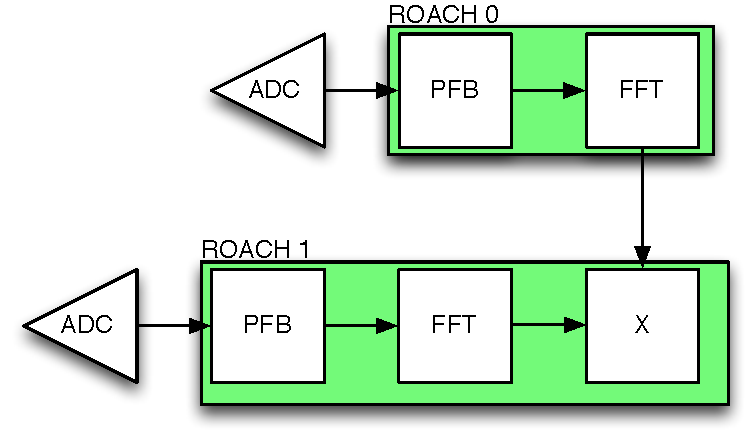
\includegraphics[width=0.48\textwidth]{Images/C5/symmetrya.pdf}
     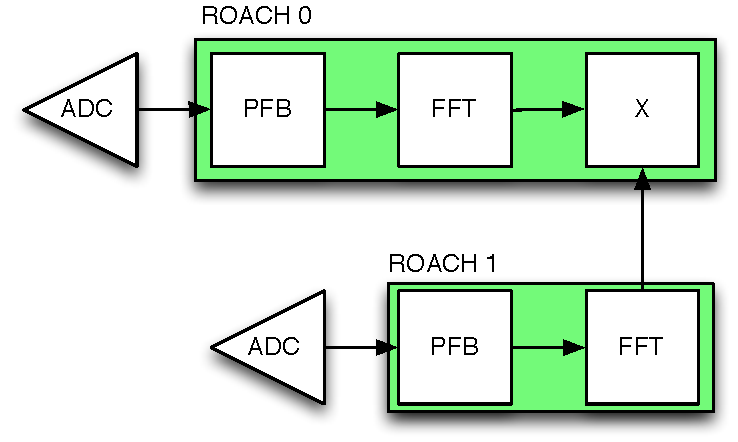
\includegraphics[width=0.48\textwidth]{Images/C5/symmetryb.pdf}
  \caption{Example of Design Symmetry in the ILP}
  \label{fig:C5/symmetry.pdf}
\end{figure}

% F Margot. Symmetry in integer linear programming. 50 Years of Integer Programming 1958-2008, pages 647�686, 2010. 
In this type of program, symmetry significantly increases the amount of time required to confirm an optimal solution.  %TODO: what type of program?
The boards that have the same platform type are interchangeable, so if board $i$ implements some design and board $j$ implements a different design in the optimal solution, there is another optimal solution where their designs are swapped.
% TODO add example (?)
% TODO add a graphic for this example
For example, suppose 2 ROACH boards are available to implement a FIR filter and an FFT. 
The ILP might observe that both blocks cannot fit on a single board and assigns the FIR to the first ROACH and the FFT to the second ROACH.
This obviously seems like an optimal solution, but the ILP may also need to check the case where the FFT is placed on ROACH\_0 and the FIR is on ROACH\_1, only to find that it has the same cost as the previous result.
In this simple example there was only one other solution to search, but as the ILP and the search space grows the number of solutions that are symmetric to the optimal case will also grow. %TODO: est of how fast?

%TODO: Figure descr

Searching symmetric solutions can become a major time sink, because the ILP solver may find an optimal solution early on, but will require a long time to confirm that it is actually the optimal result, spending time going over many other solutions that are isomorphic to the first one. 


% Early stopping (non-optimal result)The simplest solution is stopping the ILP solver before returns an optimal mapping. 
This returns the current best result the solver knows of, but it cannot guarantee that the solution is globally optimal or, in the case where it is not the a globally optimal mapping, determine if it is close to the optimal solution, (determining that is analogous to solving the ILP).
Early stopping works well when it's clear that symmetry is the cause of the long runtime and the amount of time it would take to get one of the isomorphic optimal solutions is short. 
Even so, the lack of predictable and repeatable results makes early stopping an unappealing solution.

%TODO: subset mapping

% Break symmetry - this is a good idea
The solutions above outline ways to cope with the existing symmetry. 
Another way to reduce the runtime is to remove the symmetry altogether. 
In order to do this, the ILP must be modified so that only 1 of the isometric optimal solutions is a valid solution to the ILP. 
First, a variable $lex\_order_i$ is added for each board.
This variable is meant to uniquely identifies the design running on the board; it is simply the concatenation of all the $n_{i,b}$ variables for that board.
Note that the ordering of $n_{i,b}$ variables when the concatenation is done is irrelevant, the only thing that matters is that the order is consistent for every board.
When $lex\_order_i =lex\_order_j$ we can infer that for all blocks $b$, $n_{i,b} = n_{j,b}$.
Otherwise, there must be some block $b$ where $n_{i,b} \neq n_{j,b}$.
Now that the designs can be identified, they can be ordered. 
They are simply ordered lexicographically, by adding the constraints in Equation \ref{eqn:leq_constraint} for every $i \geq 1$

\begin{align} \label{eqn:leq_constraint}
lex\_order_{i-1} \geq lex\_order_i
\end{align}

While this make the ILP, adding both constraints and variables, it reduces the amount of time the solver takes to find a solution. %TODO add a benchmark if feasible (?)
This lexicographic ordering makes it impossible to swap designs between different blocks, resulting in unique and valid mappings. 

Revisiting the symmetry example at the beginning of this section, the design with 1 FIR and no FFTs would be encoded with a $lex\_order = 10$, and the design the no FIRs and a single FFT would get the encoding $lex\_order = 01$. 
When the FIR is placed on ROACH\_0, then $lex\_order_0 = 10 \geq lex\_order_0 = 01$, satisfying the new constraint.
The solution where the blocks are swapped and FIR is on ROACH\_1 violates the new constraint  $lex\_order_0 = 01 \not \geq lex\_order_0 = 10$, and will not be considered by the ILP solver.

Generalizing this, it is impossible to take a valid solution (with the lexicographic constraint) and get another valid solution by swapping distinct designs between boards.
Suppose, without loss of generality, board $i$ has a design with $lex\_order_i = x$ and board $j$ has a distinct design with $lex\_order_j = y$ and $i < j$.
Knowing that the design is valid implies $x \geq y$. 
Another optimal mapping exists where the designs are swapped and $lex\_order_i = y$, $lex\_order_j = x$, but we are guaranteed that this is not a valid solution to the ILP because it violates the lexicographic ordering constraint.

These constraints have been implemented in the final ILP and drastically reduces the amount of time it takes to solve the ILP. 
The additional constraints do not change the cost of the optimal solution, instead they just reduce the number of valid optimal solutions. 
By modifying the ILP, the performance is greatly improved without sacrificing optimality or usability.

%Here's how we do it. 
%TODO: add google ref that talks about lex ordering

%# impose an ordering on the boards, this doesn't do anything to the solution, just breaks some of the symmetry
%        #lex_order[currentplatform,currentboard]=LpVariable('lex_order_'+unique_id,0,(maxblockperplatform+1).prod(),LpInteger)
%prob+=board_isused[currentplatform,currentboard-1]>=board_isused[currentplatform,currentboard]
%            prob+=lex_order[currentplatform,currentboard-1]>=lex_order[currentplatform,currentboard]
%           




\section{Final Mapping}
%Variables
%Design choices
The final mapping produced by the ILP is just a list of variable indicating which blocks go on which boards and the cost of the design.
Figure \ref{fig:C5/mapped_dataflow.png} shows an example of the output produced by ORCAS.
The design is a simple wideband spectrometer model.
The mapping indicates that the design will use one ROACH board and two GTX 580 servers, placing the FIR and coarse FFT on the FPGA and the remaining fine FFTs on the GPU.

\begin{figure}[ht!]
  \centering
     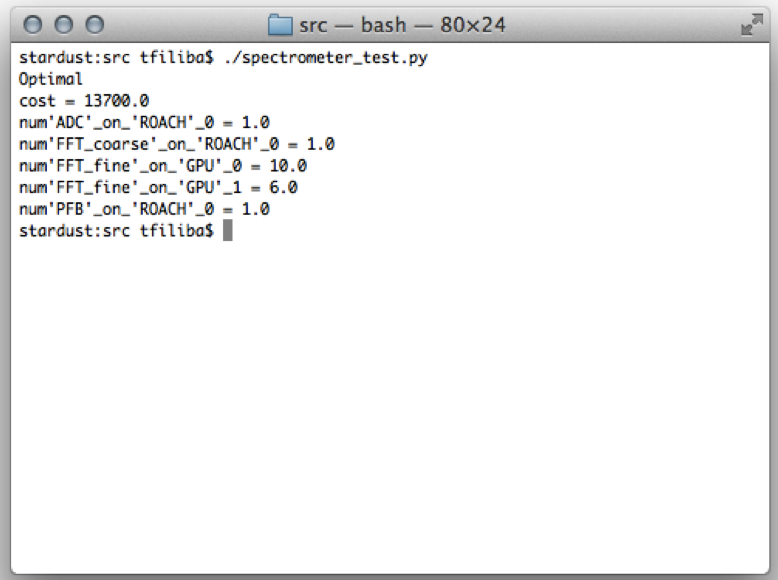
\includegraphics[width=0.75\textwidth]{Images/C5/mapped_dataflow.png}
  \caption{ORCAS Output}
  \label{fig:C5/mapped_dataflow.png}
\end{figure}

